\chapter{算法实现的一些细节}

\section{基本的数据操作和数据结构}
在四面体网格$\tau$的数据结构以及其上的数据操作是我们整个算法中最基础也是最重要的部分。因此,我们根据我们的需求,寻找或设计一个简单高效的四面体网格数据结构。通过对我们的算法整个过程的分析,我们将$\tau$上的数据操作分为查询和修改两类。在$\tau$上的基本查询有:遍历$\tau$上的所有顶点、所有边和所有四面体;查询一个顶点一环邻域的四面体,查询一个四面体上所有的顶点。修改操作有:添加或删除顶点;添加或删除四面体。最简单的情况下,我们可以直接用两个矩阵(一个$n \times 3$的矩阵用来存储顶点坐标,和一个$n \times 4$的矩阵用来存储四面体所包含的顶点索引)来表示一个四面体网格的数据。但是在我们的整个算法的过程中需要不断地查询脱皮信息,并改变$\tau$的拓扑结构(消边操作),这种简单的数据结构不利于我们消边操作的高效实现。受到三角网格half-edge思想的启发,针对于多面体网格的高效查询,Michael Kremer等人设计了一种half-face多面体网格结构——OpenVolumeMesh\cite{open-volume-mesh}。在half-face多面体网格结构中,包含四层基础的数据结构:vertex、half-edge、half-face和cell(多面体单元)。同时,half-face多面体的数据结构中包含两类关系信息:由上到下的关系信息和由下到上的关系信息(如图\ref{fig:half-face-top-down})。由上到下的关系信息是指对于除顶点外任意一层的元素,都包含一个用来构成它的下一层元素的一个有序列表(cell包含一个half-face的列表,half-face 包含一个half-edge的列表,half-edge包含一个vertex的列表)。由下到上的关系信息是指对于除多面体外的任意一层的元素,都包含一个需要用它来构成的更上一层的元素的有序列表(如图\ref{fig:half-face-down-top},vertex包含half-edge的一个列表,half-edge包含一个half-face的列表,half-face包含cell的列表)。另外在half-face多面网格的数据结构中,对于half-edge和half-face的每个元素中还保存了与其对立的那个half-edge和half-face。\par
\begin{figure}[htbp]
    \centering
    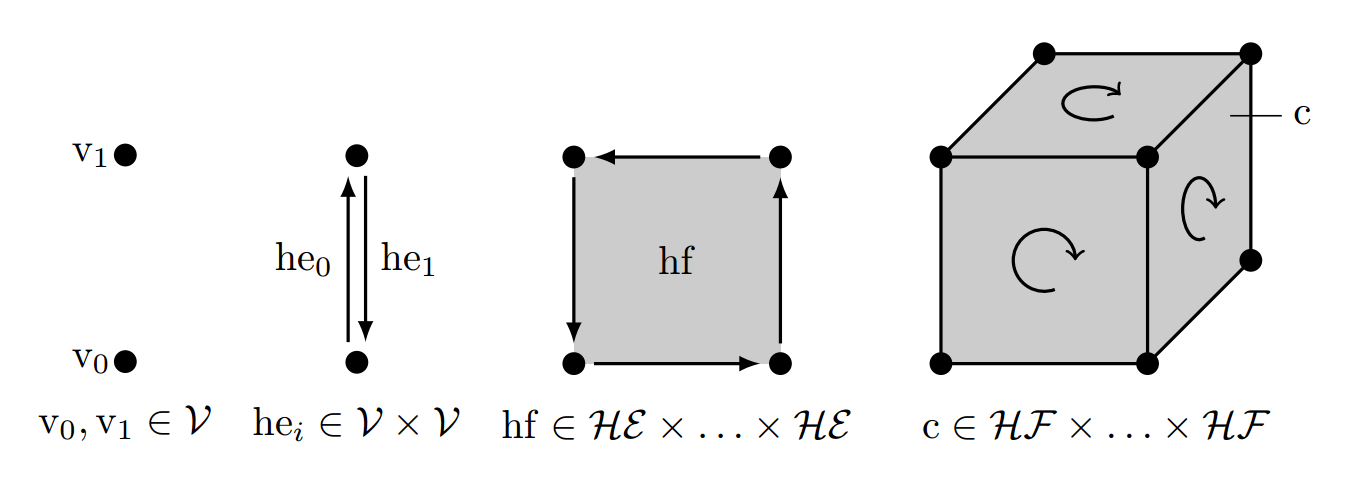
\includegraphics[width=.7\textwidth]{half-face_top_down.png}
    \caption{从上到下的关系信息示意图,对于除顶点外任意一层的元素,都包含一个用来构成它的下一层元素的一个有序列表,这些下层元素的排列顺序,决定了这个上层元素的朝向。图来自\cite{open-volume-mesh}}
    \label{fig:half-face-top-down}
\end{figure}

\begin{figure}[htbp]
    \centering
    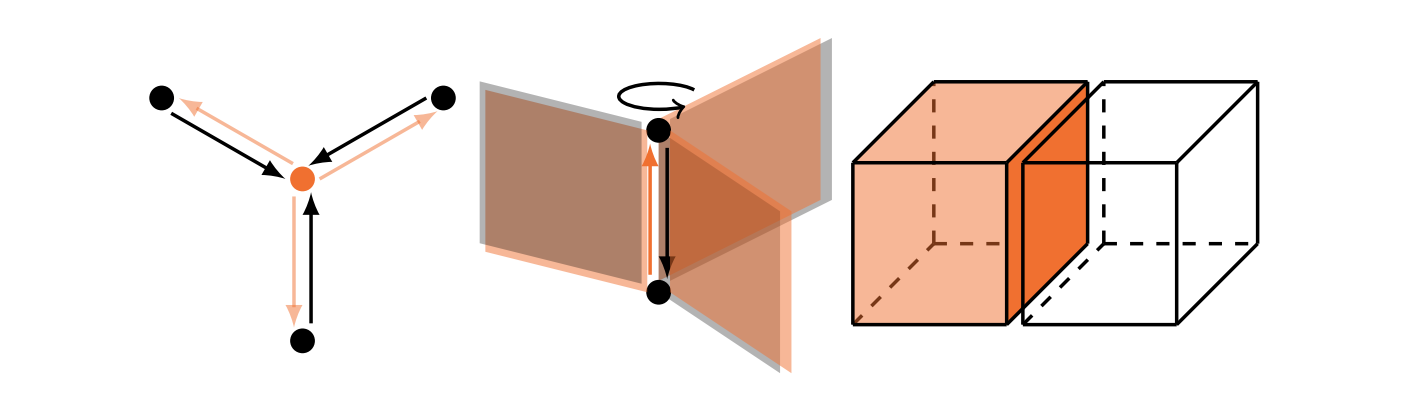
\includegraphics[width=.7\textwidth]{half-face_down_top.png}
    \caption{从下到上的关系信息示意图,对于除多面体外的任意一层的元素,都包含一个需要用它来构成的更上一层的元素的有序列表。图来自\cite{open-volume-mesh}}
    \label{fig:half-face-down-top}
\end{figure}
从上面half-face多面体网格的数据结构的描述中,我们可以看到,邻接信息的存储非常到位,对于任意一层的元素通过很少的查询,就能找到与其相邻的任意一层的元素列表,也就是说在half-face这个数据结构上信息的查询操作非常高效(比如查询一个顶点的邻接点,查询一个面的邻接多面体等等)。然而对于消边操作,由于需要维护很多的邻接关系,不仅复杂而且非常低效。\par
幸运的是,CGAL不仅给我们提供了鲁棒可靠的3D Delaunay三角化算法,而且给我们提供了一种很号的四面体网格数据结构Triangulation\_3d,其能够非常好地满足我们的需求——简单高效。在 CGAL的四面体数据结构(如图 XXX)(graphvz 类图)中,包含两种最基本的数据:顶点和四面体,而边和面则通过四面体和顶点的组合来表示。对于每一个四面体,存储了该四面体的四个顶点的handle和分别与其四个面相邻接的四个四面体的handle;对于每一个顶点,存储了包含该顶点的某一个四面体的handle。通过这个简单的拓扑关系,我们就能够较为高效地查询出该四面体网格上的邻接信息,而且在做消边时也能够较为高效地维护该数据结构。

\section{密度为$\sigma$的均匀采样}
对于三角形上密度为$\sigma$的均匀采样,一种简单的均匀采样方法是为三角形做一个从全局到局部的坐标变换,使得一条边在x或y轴上,然后在其包围矩形上均匀采样,并选取属于这个三角形内的采样点(如图 XX)。但是这种方法并不鲁棒,对于有些三角形,该方法无法保证密度为$\sigma$这个条件——即以每个采样点为圆心,以$\sigma$为半径的圆能将这个三角形全部覆盖。为此,我们想出了一种更好地采样方法:我们知道对于$\triangle ABC$中的任意一个采样点s都可以表示为:
\begin{equation}
  \begin{split}
    s = \lambda_0 \overrightarrow{AC}+\lambda_1 \overrightarrow{AB} + A\\
    \lambda_0 + \lambda_1 \leq 1, \quad \lambda_0 \geq 0, \quad \lambda_1 \geq 0
  \end{split}
\end{equation}
因此,我们可以通过对于$\lambda_0$和$\lambda_1$分别取$\frac{\sigma}{\parallel \overrightarrow{AC} \parallel}$的采样密度,得到$(\lambda_0,\lambda_1)$的采样,从而间接计算得到$\triangle ABC$上密度为$\sigma$的均匀采样(如图XX)。
